\documentclass[11pt,a4paper]{jsarticle}
	\usepackage{amsmath,amssymb}
	\usepackage{amsfonts}
	\usepackage{bm}
	\usepackage[dvipdfmx]{graphicx}
	\usepackage{ascmac}
	\usepackage{okumacro}
	\usepackage{titlesec}
	\usepackage{here}%画像を強制的に指定場所に置く[Here]を使える
	\usepackage{cases}%連立方程式など
	\setlength{\textwidth}{\fullwidth}
	\setlength{\textheight}{39\baselineskip}
	\addtolength{\textheight}{\topskip}
	\setlength{\voffset}{-0.5in}
	\setlength{\headsep}{0.3in}
	%
	\makeatletter
	\def\section{\@startsection {section}{1}{\z@}{-2.5ex plus -1ex minus -.2ex}{2.5 ex plus .2ex}{\LARGE\bf}}
	\def\subsection{\@startsection {subsection}{1}{\z@}{-1.5ex plus -1ex minus -.2ex}{2.3 ex plus .2ex}{\Large\bf}}
	\def\subsubsection{\@startsection {subsubsection}{1}{\z@}{-2.5ex plus -1ex minus -.2ex}{.3 ex plus .2ex}{\large \bf}}
	\makeatother

	\makeatletter
	    \renewcommand{\theequation}{%
	    \thesection.\arabic{equation}}
	    \@addtoreset{equation}{section}
	  \makeatother


	\newcommand{\divergence}{\mathrm{div}\,}  %ダイバージェンス
	\newcommand{\grad}{\mathrm{grad}\,}  %グラディエント
	\newcommand{\rot}{\mathrm{rot}\,}  %ローテーション
	\newcommand{\pt}{\partial}  %パーシャル
	\newcommand{\df}{\overset{\mathrm{def}}{=}} %def
	\newcommand{\non}{\nonumber}  %\nonumber
	\newcommand{\dis}{\displaystyle}
	\newcommand{\f}[1]{\framebox[1cm]{\textgt{\small #1}}}
	\newcommand{\kine}{\frac{1}{2}mv^2} %運動エネルギー
	\newcommand{\sceq}{Schrödinger equation}
	\pagestyle{plain}
		%\markright{\footnotesize \sf 物理数学1A 第一回中間テスト(2017) 解答例 \ %左上のタイトル
		%{@sakuPonit}} %名前
\begin{document}

%% 表紙
\begin{center}
    \huge 平成30年度 物理学実験(二)\par
    \vspace{15mm}
    \Huge プランク定数 \par
    \vspace{60mm}
    \Large  実験日: 平成30年5月28日\par
    \vspace{15mm}
    \Large 1217054 佐久間寛伸\par
    \vspace{10mm}
  \end{center}
  \thispagestyle{empty}
  \clearpage
  \addtocounter{page}{-1}
  \newpage

%% 目次
\tableofcontents
  \newpage

%% 内容
\section{はじめに}
	\ 本報告書では書籍等からの引用をしている箇所がある.その被引用部で
	式番号が振られていた場合,本報告書内での式番号と重複・前後しないよう筆者がレポートの章立てに合うように適宜振り直しをした.
	そのため本報告書と引用元とでは式番号が異なることに留意されたい.
\section{目的}
	\ プランク定数測定器により,ハロゲン灯の光を分光し,振動数が知られているいくつかの単色光と
	Sb-Cs光電管とを用いて光電効果(photo-electric effect)の実験を行なう.それらの結果から,
	光が粒子性を示すことを理解し,
	さらにプランク定数(Planck constant)$h$を求める.

\section{原理}
	\subsection{プランク定数とエネルギー量子}
		\ そもそもプランク定数とは「量子力学的な現象を特徴づける普遍定数.
		ドイツの物理学者プランクが熱放射の研究のなかで1900年に発見した.」 \cite{planckconst01}物理定数である.
		ここでは『発見した』とあるが,
		「M.プランクは空洞放射の測定値を十分説明できる関係式(プランクの放射式)を見出したが,
		この式を導き出すには,振動数$\nu$の振動子のエネルギーの放出・吸収が連続的ではなく,
		$h \nu$を単位とする不連続な量の放出・吸収だけが許される,と仮定せざるをえなかった.
		ただし,$h$はプランク定数である.」 \cite{planckconstブリタニカ}
		のような,定数を『仮定』したという表現が適切と考える.
		\par また,『$h\nu$を単位とする不連続な量』をエネルギー量子(energy quantum)
		といい,これについては
		「$h \nu$をエネルギー量子という.エネルギー量子の考えは,
		エネルギーの連続性を根本的な足場にしている古典物理学の自然観と正面から対立し,
		量子論を生み出す第一歩となった.この功績により,1918年プランクにノーベル物理学賞が授与された.
		プランクのエネルギー量子という考えは,A.アインシュタインによって光量子という考えに発展した.」
		\cite{planckconstブリタニカ}
		とあるように光電効果,ひいてはそれ以降の量子論に繋がる重要な概念である.

	\subsection{光電効果}
		\ 光電効果については
		「金属の表面に光を照射すると電子が飛び出す.この現象を光電効果(特に外部光電効果)といい,
		飛び出した電子を光電子(photo-electron)と呼ぶ.アインシュタイン(A. Einstein)は,
		1905年にプランク(M. Planck)のエネルギー量子の考え方を発展させ,
		振動数$\nu$の光が伝播することは$hv$のエネルギーを持つ粒子が空間を
		飛んでいくことであると考えた.ここで$h$はプランク定数である.このような光の粒子を光子または光量子
		(photon)と名付けた.光電効果は,光子が金属中の電子と衝突してそれが持っているエネルギーを一度
		に全部電子に与え,その結果電子が金属の表面から外に飛び出す現象と解釈される.したがって,電子が金
		属表面を越えて外に出るために要する最小のエネルギーを$E$とすると,飛び出した光電子が持つことのでき
		る最大の運動エネルギーEは
			\begin{equation}
				E = h\nu - e\varphi \label{workfunc01}
			\end{equation}
		である.ここに$e$は電子の電荷の符号を変えたもので,素電荷と呼ばれる.
		また$\varphi$は仕事関数(work function)とよばれ,金属の種類によって決まる.
		\par 式(\ref{workfunc01})で$E=0$,つまり
			\begin{equation}
				\nu_0 = \frac{e \varphi}{h} \label{threshold frequency}
			\end{equation}
		を満たす振動数$\nu_0$を限界振動数という.
		限界振動数以下の振動数$\nu \leq \nu_0$の光は,それがどんなに強くても,
		その金属表面から電子を飛び出させることはできない.」
		\cite{物理学実験}
		とある.
		\par また,光電流については以下のように説明されている.「光電管(photon-tube)に振動数が$\nu$の単色光を入射すると,受光面である陰極から電子が飛び出すので,
		この陰極(受光面) と陽極を結ぶ外の回路に電流が流れる.
		この電流を光電流(photo-current) と呼ぶ.」
		\cite{物理学実験}
		\par さらに,光電効果を利用してプランク定数を求める方法については
		以下の通りである.
		「このとき,陽極側が負になるように電圧をかけ,
		その電圧を増加して行くと,光電流は減少する.
		この負電圧と光電流の関係を表す曲線を外挿して
		光電流がゼロに対応する負電圧をもとめる.
		このとき,光電子がどんな運動エネルギーを持っていても,全て陰極に押し返されている.
		したがって,この負電圧を$-V_0$とすると,
		$E=eV_0$であるから,式(\ref{workfunc01})は,
			\begin{equation}
				eV_0 = h\nu - e\varphi \label{workfunc02}
			\end{equation}
		となる.いくつかの振動数\nuについて同様な測定を行い,$\nu$と$eV_0$の関係を求めると,それは直線となり,その
		勾配からプランク定数$h$が得られる.知られている$h$の値は($6.626176 \pm 0.000036) \times 10^{-34}$J \cdot{\rm s}である.\\
		また,この直線を外挿して,用いた光電管の受光面を形成している金属の表面物質の仕事関数 $\varphi$ が得られる.」
		\cite{物理学実験}
		\par なお,仕事関数について
		「光が$h\nu$のエネルギーを持つ粒子であることから,単色光を指定する場合に波長や振動数のほか,光子エネ
		ルギー(photon energy)も使用される.単位としては,通常,エレクトロン·ボルト(eV)を用いる.1エレク
		トロン·ボルト= $e \times 1 $ジュールである.」
		\cite{物理学実験}
		とある.筆者は高校生時代に「仕事関数$W$の単位はJである.」と習ったが,
		「仕事関数は電子ボルトを普通は単位と」する\cite{planckconstブリタニカ}ことを
		明示的に記しておく.また,


\section{実験}
	\subsection{実験課題}

	\subsection{実験装置}
		\subsubsection{分光器}
			\  本実験で用いたプランク定数測定器は島津理化製HA-30A(図\ref{fig1})であり,製造元によると
			「島津独自のホログラフィックグレーティングを用いたモノクロメータは,純度の高い単色光を取り出せます.」
			\cite{ha30a}とあるが,ホログラフィックグレーティング(ホログラフィック回折格子)とは,基板上のフォトレジスト(光に反応し物性を変える)を2本のレーザの光干渉により正弦波状に形成することで作成されるグレーティング(回折格子)である.
			\cite{ホログラフィックグレーティング}
			\cite{島津回折格子}
			\par なお「島津独自の」という部分に関して,
			島津理化のホログラフィックグレーティングは独自技術によりブレーズ化が施されており
			ブレーズ化されていない回折格子に比べ
			特定の次数と波長に対して高い回折効率を示すという特長をもっている.
			ブレーズ化された,つまり溝の断面形状が鋸歯状である回折格子(ブレーズド回折格子)は,
			溝本数$N$,入射光の波長$\lambda_B$,取り出す回折光の次数$m$が決まっている場合,
			入射角を変化させ特定の入射角$\alpha$にすることで回折効率を高めることができる.
			この関係を満たすブレーズド回折格子の溝の傾きをブレーズ角$\theta_B$と呼び,
			入射光の波長$\lambda_B$をブレーズ波長と呼ぶ.$\lambda_B$は以下の式(\ref{ブレーズ波長})により求められる.
				\begin{equation}
					\lambda_B = \frac{2}{Nm} \sin{\theta_B} \cos{(\alpha - \theta_B)}
					\label{ブレーズ波長}
				\end{equation}
			この特性を用いて,本実験ではプランク定数測定器の"角度目盛盤"を操作し
			入射光に対するグレーティングの角度を変化させ,特定の単色光,つまり特定の波長を取り出す.



			\begin{figure}
						\begin{center}
							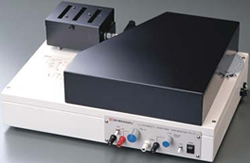
\includegraphics[width=80mm]{eqp01.jpg}
						\end{center}
						\caption{HA-30A \cite{ha30a}}
						\label{fig1}
					\end{figure} %HA-30A

	\subsection{実験手順}


\section{結果}

\section{考察}





%% 参考文献
\begin{thebibliography}{9}
  \bibitem{planckconst01}江沢洋 『日本大百科全書(ニッポニカ)』 小学館
  \bibitem{planckconstブリタニカ}『ブリタニカ国際大百科事典 小項目事典』 ブリタニカ・ジャパン
  \bibitem{物理学実験}東京理科大学 理学部第一部 物理学教室 『物理学実験(二)』 (2018)
	\bibitem{ホログラフィックグレーティング}Palmer, Christopher, {\sl Diffraction Grating Handbook}, 6th edition, Newport Corporation (2005)
	\bibitem{島津回折格子}島津理化HP 製品情報 - 回折格子(グレーティング)の解説
	\bibitem{ha30a}島津理化HP 製品情報 - プランク定数測定器 HA-30A
	\bibitem{レタス}プランク定数測定器の取扱説明書 (https://letus.ed.tus.ac.jp/course/view.php?id=81223)
	\end{thebibliography}

\end{document}
